\documentclass[12pt]{article}
\usepackage[margin=3cm]{geometry}
\usepackage{blindtext}
\usepackage{chngcntr}
\counterwithin*{section}{part}
\usepackage{enumitem}
\usepackage{listings}
\usepackage{float}
\usepackage{graphicx}
\usepackage{soul}
\usepackage{tikz}
\usepackage{subfig}
\usepackage{hyperref}
\usepackage{amsmath}
\usepackage{tabularx}
\usepackage{multicol}
\usepackage{tcolorbox}
\usepackage{xcolor}
\lstset{language=C++,
    basicstyle=\ttfamily,
    keywordstyle=\color{blue},
    stringstyle=\color{red},
    commentstyle=\color{green},
    morecomment=[l][\color{magenta}]{\#}
}

\hypersetup{
    colorlinks=true,
    linkcolor=black,
    citecolor=green,
    urlcolor=red
}
\usetikzlibrary{quotes, angles, decorations.markings, intersections}
\usetikzlibrary{calc,patterns,angles,quotes, 3d, intersections, positioning, shapes, automata, positioning}
\newcommand{\tbox}[1]{\noindent\fbox{\parbox{\textwidth}{#1}}}
\title{Networks CS348 Notes}
\author{}
\date{\today}

\begin{document}

\maketitle
\tableofcontents

\setlength{\parskip}{6pt}
\setlength{\parindent}{0pt}

\setlist[itemize]{topsep=0cm,parsep=0cm,itemsep=0cm}
\setlist[enumerate]{topsep=0cm,parsep=0cm,itemsep=0cm}

\newpage
\noindent\tbox{
    \begin{center}
    \textbf{\Huge Lecture 1}
    \end{center}
}
\part{General Ideas}
\section{Introduction}
What is a computer network? A computer network is a group of interconnected devices that can exchange data and resources with each other.
\st{Almost} all of today's devices are in one way or another connect the biggest computer network alias the Internet. There are several 
abstractions and nuances that enable the existence of such a huge structure.

A network consists of several end hosts which are systems that request/receive data using the network. These end hosts are connected 
using links which can directly connect the hosts together or more commonly connect multiple of them to switches/routers which can 
simplify the network while still providing connectivity among hosts. 

\subsection{Topologies}

A group of hosts can be connected in multiple ways. The type of graph that is obtained from considering the 
hosts as nodes and links as edges is called the `topology' of that network. 
Some examples include a bus where all hosts are connected to a common wire. Others include star topology where hosts are connected to a central host. 

Links can also be classified on the basis of how many users can communicate across them.
\begin{itemize}
    \item \textbf{Simplex:} Only one user can talk across a link
    \item \textbf{Duplex:} Both users can communication \textit{simultaneously} across a network. 
    \item \textbf{Half Duplex:} Both users use the same link to communication but not simultaneously. 
\end{itemize}

\begin{figure}
    \centering
    \begin{minipage}{.5\textwidth}
      \centering
      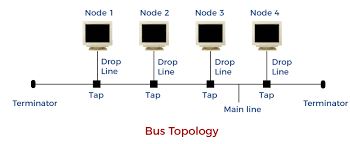
\includegraphics[width=0.9\linewidth]{Diagrams/bus.png}
      \captionof{figure}{Bus Topology}
      \label{fig:test1}
    \end{minipage}%
    \begin{minipage}{.5\textwidth}
      \centering
      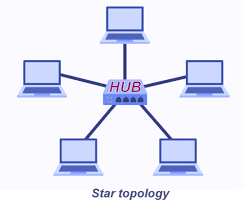
\includegraphics[width=.45\linewidth]{Diagrams/star.png}
      \captionof{figure}{Star Topology}
      \label{fig:test2}
    \end{minipage}
\end{figure}


\subsection{Switch}
What exactly is a switch? The Switch is a network device that is used to segment the networks into different subnetworks called subnets. It can help simplify a 
network by grouping together lots of hosts into a sub-network. A switch has multiple incoming and outgoing links. It is capable of 
routing data from an incoming link to an appropriate outgoing link.

\begin{figure}[H]
    
    \begin{center}
    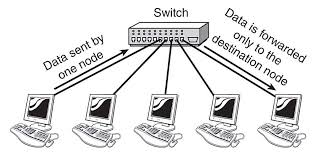
\includegraphics[width = 8cm]{Diagrams/switch.jpeg}
    \end{center}
    \label{fig:switch}
    \caption{Example of a switch}
\end{figure}
\section{Abstractions, Layering in a network}

There is always the possibility to deal with the network as a single structure at once. That is 
to deal with the entire flow of data from the second a request is made by a `user' and all the way till 
the request is serviced in one go. 

However, this is very inconvenient and complicates the network in the sense that any change made to some part of the network can make or break the entire system. 
To combat this the network is clearly split into layers where each layer operates relatively independently and only exposes parts of it that 
are necessary for the higher and lower layers in the network. 

To better understand this let us take an example.

The most common request on the Internet is an HTTP request (ie) a request by a computer for a webpage. Let us see the flow of information when such a request is made.

\begin{enumerate}
    \item \textbf{Application layer:} The URL is entered into a browser and then a user request is made. Then this URL is converted into the \textbf{IP}\footnote{will be dealt with later, assume it is some id for a computer} address of the server
    that holds the page needed by the user. 
    \item \textbf{Transmission layer:} Now that we know the IP address from the application layer, the request for a page is sent to that address using the transmission layer. This layer sends the 
    request message in manageable pieces to the network to be sent to the web server. 
    \item \textbf{Network layer:} Now these `manageable pieces' need to be sent to the destination (ie) web server. The next router/link to which the message is to be sent 
    is decided in this layer. These links `talk' to each other in some sense and know where to send messages to reach the web server. 
    \item \textbf{Data Link layer:} The data link layer deals with splitting the message bit by bit and choosing the appropriate media to transfer them using (ie) Optic fiber, Wireless links etc..
    \item \textbf{Physical layer:} Finally the physical layer deals with transmitting the actual bit signals over whatever media is chosen.
\end{enumerate}


Now once the data is transferred to the physical layer of the web server, it climbs up in the layers till the application layer of the web server is reached. The response of 
the web server is transmitted back similarly. This by no means completely covers the functionality of each layer but rather gives a flavour of each layer's functions. It is easy to see 
how the abstraction is helpful as now the application layer has no need to worry about which media is used to transfer the bits 
and the Physical layer is oblivious to what message it is transferring. 

The abstraction helps to simplify the structure of the network by helping us deal with one subproblem at a time. 



\noindent\tbox{
    \begin{center}
    \textbf{\Huge Lecture 2}
    \end{center}
}


\subsection{IP address}

Each connected device has a unique identifier to describe it.
This identifier is known as the IP address of a device. 

The IP address has a hierarchical structure. An example of an IP address is `72.85.5.25'. This can be thought of 
as being similar to a postal address where the country of your address is the highest level at which location is specified. 
After this the state, city, area narrow down your location more and the message travels in an organised way from one `level' to another.

In fact as discussed before each router at the Network layer transmits a message to a particular router which is chosen based on its IP address and the IP address of the destination. 
How is this rerouting done?

\begin{itemize}
    \item \textbf{Readjusting weights:} The weights of each connection can be adjusted to change the shortest path to the destination
    \item \textbf{Longest Prefix Match (Practical):} There is a router table present which gives us the IP corresponding to a router. When a packet has to make the choice between routers it takes the router connected to the
    current router with the longest prefix match when compared to the destination address. 
\end{itemize}

\subsection{Message Granularity, Delays}

The size of the message which is being sent via the network changes depending on which layer the transfer happens in.
That is a message can be described in various granularities.
\begin{itemize}
    \item \textbf{Application layer}: Application dependent, a video/ a webpage etc..
    \item \textbf{Transmission layer}: TCP splits the message into segments, UDP splits it into Datagrams
    \item \textbf{Network layer:} Transfers data as packets
    \item \textbf{Data Link layer:} Symbols
    \item \textbf{Physical layer:} Bit by Bit
\end{itemize}


As we saw in the last Lecture a router has some number of `in' connections and `out' connections which are connected together depending on which 
`out' connection the message is supposed to be sent. This  `routing' is done by putting each incoming packets on queues corresponding to the outgoing connection we 
are supposed to send to.

This rerouting is done so that if the incoming rate to an out connection is greater than its outgoing rate we have the queue as a buffer.


Why do we just not make the queue very large to prevent these 'drop offs'
\begin{itemize}
    \item \textbf{Cost:} Memory is not free so we need to be aware of the trade offs of increasing the queue size
    \item \textbf{End-End delay:} If the router has a buffer of say size $Q_{max}$ and an output rate of c $bits/sec$.
    Now if the queue is almost full and we get a new packet put in at the very end, the packet takes $\frac{Q_{max}}{c}$ time to be put on the next connection. 
    This is called the End-End delay and clearly a large queue increasing the worst case End-End delay
\end{itemize}

The total delay for a transmission of a packet through some K routers would be 
\[ Delay = \sum_{k = 1}^{k = K}\frac{Q_{max}^k}{c^k} + S_d + T_d\]

\(S_d\) is called the speed of light delay and \(T_d\) is the transmission delay. 
In most applications End-End delay is the significant bottle neck for the whole delay. Infact in some applications 
we prefer dropping packets inorder to not have high delays\footnote{Think of voice call where a delay would lead to not being able to communicate anything}


\subsection{Layering and Design Protocols}
Any subproblem is handled by some protocol corresponding to the layer we are at. 

We have divided networks into 
5 layers. Specifically Application layer, Transmission Layer, Network Layer, Data Link Layer , Physical Layer.  
This abstraction enables users to interact only with the layer they are concerned with in that layer without having to deal with the 
network as a whole. 

Some advantages of layering networks are:
\begin{itemize}
    \item \textbf{Ease of development:} Only certain problems need to be dealt with at each layer
    \item \textbf{Debugging:} Ease in fixing new problems in each layer independently
    \item \textbf{Flexibility of Physical technologies, Applications:} As an example whatsapp as an application 
    only deals with that layer of the network. It doesn't interfere/have to deal with the particular intricacies of the 
    physical technology used by their users to connect to the network.
    \item \textbf{Ease of Modification:} We need to change only a particular layer to address problems associated with it. There is no fear of breaking the system due to modifications
    made to said layer.
    \item \textbf{Choices at each layer:} Each layer can use multiple media without breaking compatability with the system. 
\end{itemize}



\noindent\tbox{
    \begin{center}
    \textbf{\Huge Lecture 3}
    \end{center}
}



Disadvantages of layering networks:
\begin{enumerate}
    \item There is some opaqueness about other layers. As an example let's say 
    a packet is sent from a source to destination using a sequence of routers. If a packet is dropped midway, 
    TCP makes an assumption that they were dropped due to a full queue. Infact there can even be wrong assumptions that a 
    packet was dropped\footnote{example for another reason is interference in wireless links}. 

    This mainly arises from the fact that the routers have little to no communication going with the protocol of a higher layer. 

    \item There is redundancy at each level of the network. \textbf{TCP} handles retransmission, but even \textbf{MAC} handles that. 
    Let's say that a packet transmission attempt in a wireless link failed. The MAC will make sure that retransmission happens. But this is also taken care by TCP which is redundant.

    \item Transmission is suboptimal. The sender of the message is unable to specify guarantees they want in the delivery of said packets. This is referred to as a 
    `Best Effort' system where the network has no guarantees regarding the quality of service
\end{enumerate}



\subsection{Latency Metrics}

\begin{enumerate}
    \item \textbf{One-Way delay:} If a packet is sent out at time $t_0$ and it reaches the destination at $t_1$, then the \textit{one way delay} of the packet is $t_1 - t_0$. However measuring 
    one day delay is difficult since it takes the direct difference in times measured at the source and destination. This difference may drift apart over time due to both systems operating at different clock cycles.
    \item \textbf{Round-Trip Time:} Once a packet is recieved by the target it sends back an acknowledgment message. The time taken from sending the messages to recieving the acknowledgment is its \textit{round trip time}. 
    
    \item \textbf{Jitter:} Jitter measures the variability in the latencies associated with the sending some \(k\) packets. Let jitter be \(J\). It can be written as
    
    \begin{align*}
    e_k &= |d_{k+1} - d_{k}| \\
    J &= \frac{1}{n-1} \sum_{k=1}^n e_k 
    \end{align*}
\end{enumerate}

\noindent\tbox{
    \begin{center}
    \textbf{\Huge Lecture 4}
    \end{center}
}

\subsection{Headers}

There is some meta data about each packet/module of data generated when a message is sent from one layer to the below layer. 
This metadata is added as a header to the message itself that is shared with the next layer. 

When a message goes to another layer below this header is not tampered with at all. Rather the next header is 
just layered on like an onion on top of the previous header. 


\begin{figure}[H]
    \centering 
    \includegraphics*[width = 10cm]{Diagrams/headers.png}
    \label{fig:headers}
    \caption{How headers are built and removed}
\end{figure}


\section{Quality of service}

There are some metrics to determine the quality of the service provided by the network. 

\begin{itemize}
    \item \textbf{Latency:} Delay from the dispatch of a packet till it reaches destination
    \item \textbf{Throughput:} Amount of data that can be sent in given time
    \item \textbf{Bandwidth:} Amount of data that can be sent at the same time in network
\end{itemize}



\part{Physical Layer}
\section{Physical Media}

\begin{enumerate}
    \item \textbf{Twisted pair cables:}
    It consits of a pair of cables twisted together (to cancel out magnetic fields created by loops). The larger the 
    number of cables and the more the twisting the better it is. 

    There are different categories of cable each having its own data transmission rates. 

    \item\textbf{Co-axial Medium:}
    Co-axial cables consist of a series of wires covered by a wire mesh to deal with magnetic fields. 
    Depending on the thickness of the mesh data transmission rates vary. 
    \item\textbf{Optic Fibre:}
    


        \begin{itemize}
            \item Single Mode: The optical fiber is so thin  that only a 
            single ray of light can cleanly pass through it
            \item Multiple Mode: A thicker fiber which is capable of transferring multiple rays 
            at the same time
        \end{itemize}


        Which of those is better? One may think it is multimode since it can transmit multiple pulses together. 
        However the rays in the multimode gets interferred with each other if they are placed closer together. 
        
        Thus there is a need to delay the throughput in multimode inorder to make sure the signals received are coherent.
        
        Overall single mode turns out to be better. 
    \end{enumerate}

\noindent\tbox{
    \begin{center}
    \textbf{\Huge Lecture 5}
    \end{center}
}

\subsection{Attenuation}

Attenuation is the loss of power when it is transmitted over a Physical media. 

\[ \text{Attenuation} = 10 \log(\frac{P_{in}}{P_{out}})\]

Attenuation has units as dB/decibels. 

Some examples on calculating Attenuation:

\begin{enumerate}
    \item  \[\frac{P_{in}}{P_{out}} = 2 \]
    \begin{align*}
        \text{Attenuation} &= 10 \log_{10}2 \\
        &= 3dB 
    \end{align*}
    \item  There are two identical wires which cause an Attenuation of 3dB. 
    The wires are connected and a signal is passed through the combined wire. Assume P1 is the power left after the signal 
    passed through one of the wires
    \[10\log_{10}\frac{P_{in}}{P_1} + 10\log_{10}\frac{P_{1}}{P_{out}} = 10\log_{10}\frac{P_{in}}{P_{out}} \]
    Thus total attenuation is the sum of attenuation of both wires.
\end{enumerate}


Another thing to be noted is that power is directly proportional to the square of the amplitude of a signal. 
Thus Attenuation can also be expressed as:
\begin{align*}
    \text{Attenuation} =& 10 \log_{10} \frac{(A_{in})^2}{(A_{out})^2} \\
    =& 20 \log_{10} \frac{A_{in}}{A_{out}}
\end{align*}
        
\subsection{Absolute Power in decibel scale}

1 mW(milli Watt) is kept as the reference to express absolute power in the decibel scale. 
That is power of P Watts can be written as \(10\log_{10}\frac{P}{10^{-3}}\). 

Absolute power has no significance to describe the quality of a transmission on its own. What does matter is Recieved power relative to Noise power. 

\subsection{Frequency vs attenuation}
\begin{figure}[H]
    \centering
    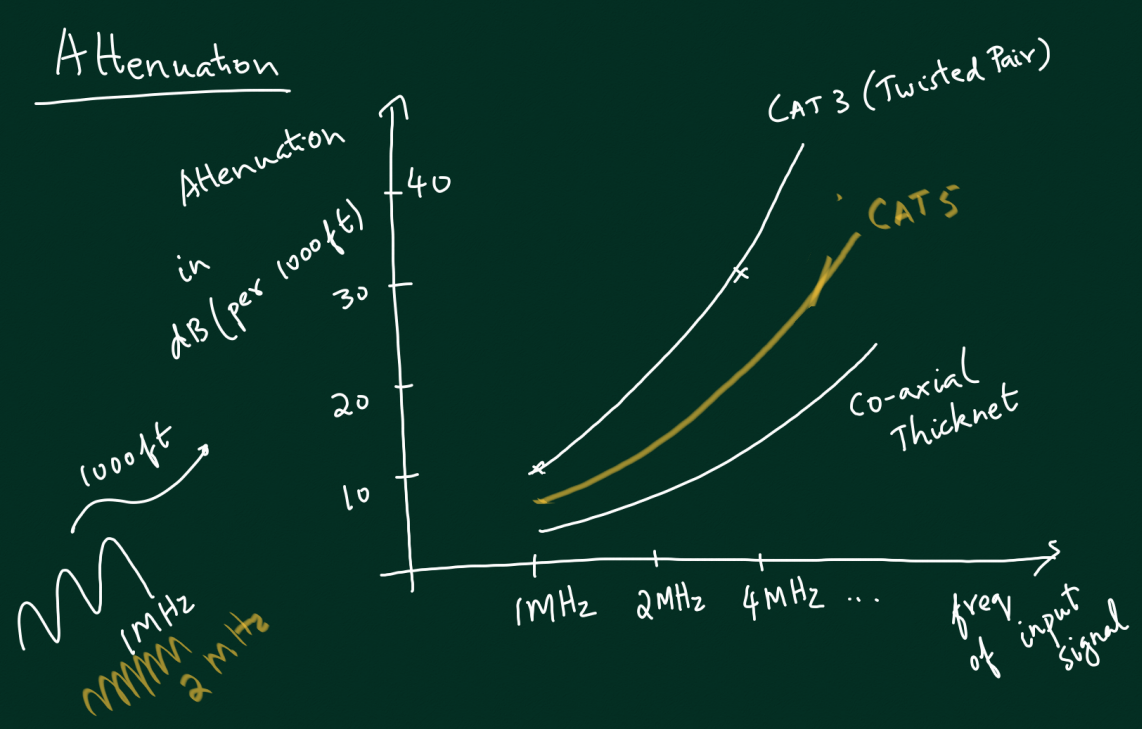
\includegraphics[width = 10cm]{Diagrams/attenuation.png}
    \label{fig:attenuation}
    \caption{Attenuation vs Length of cable}
\end{figure}
          
Clearly, attenuation increases with the frequency of the signal sent through it. 
This does not make sense considering the wire to have only resistance. Thus it is clear that the wire also has some inductance associated to make this behaviour happen. 


However, the situation is a bit different for optical fibres. 
\begin{figure}[H]
    \centering
    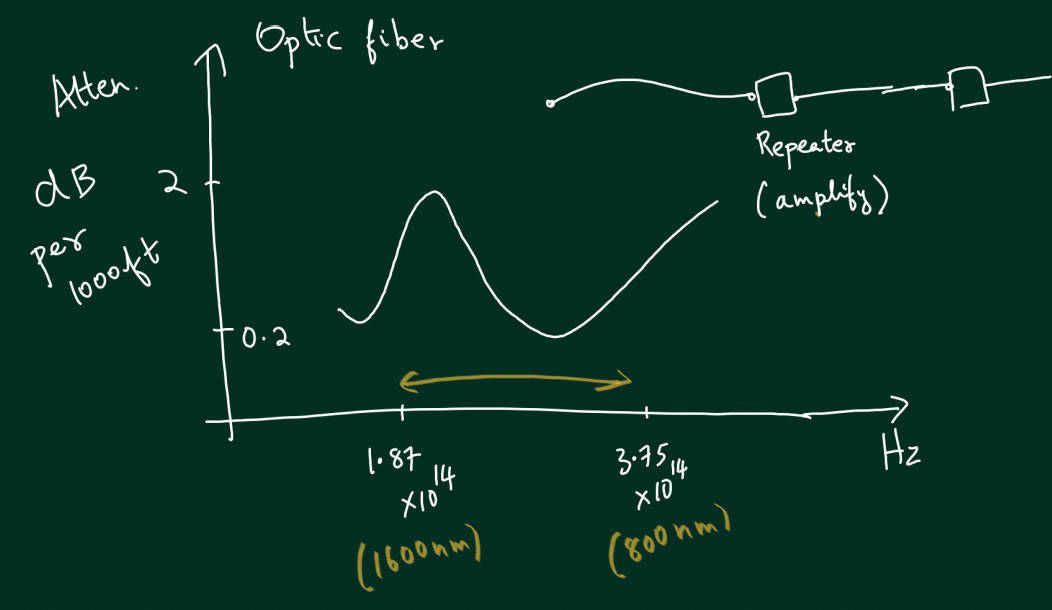
\includegraphics[width = 10cm]{Diagrams/optic_attenation.png}
    \label{fig:optic-attenuation}
    \caption{Attenuation vs Length of optic fibre}
\end{figure}

Here the attenuation shows non-linear behaviour which suggest some capacitative behaviour along with the inductance.

To prevent attenuation from decreasing signal quality, repeaters are used to boost up the signal. They are placed at calculative 
distances to maximise their advantage. 


Different signals can be sent across the same channel using a different Frequency. But 
the speed at which data can be sent decreases as the frequency range of different messages or \textbf{Bandwidth} increases. 
This can be calculated using Claude Shanon's definition of entropy. 


\subsection{Attenuation in Wireless signals}
\begin{figure}[H]
    \centering
    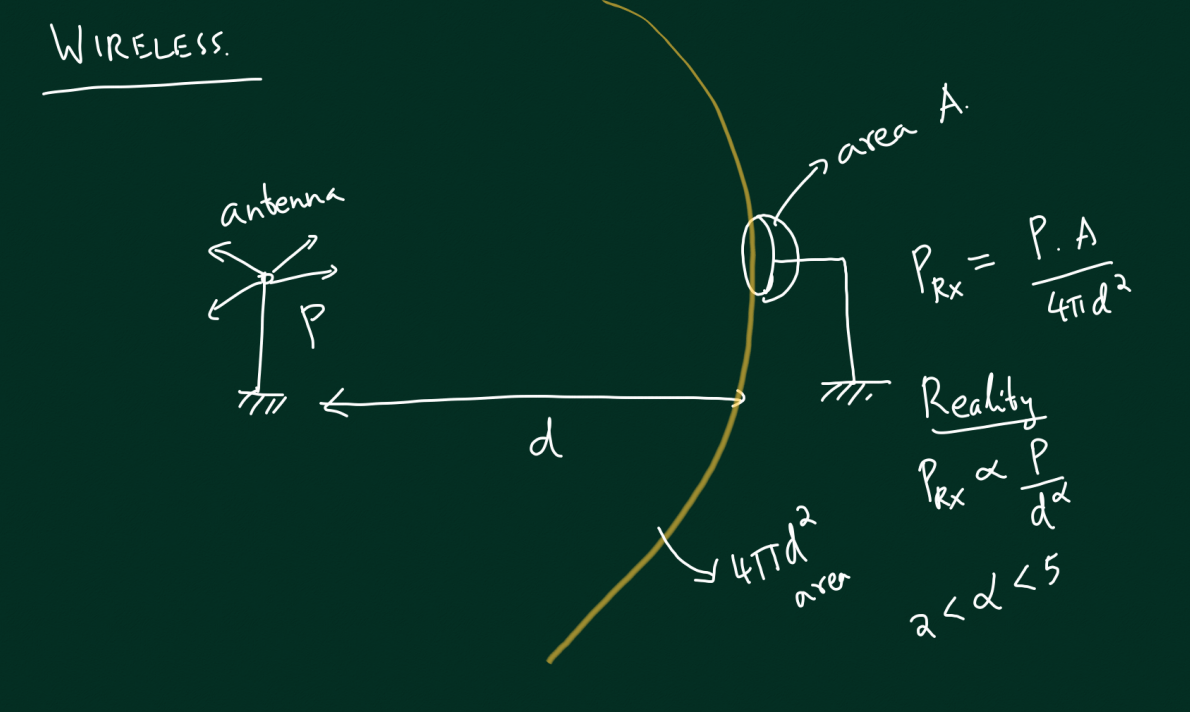
\includegraphics[width = 15cm]{Diagrams/wireless_attenuation.png}
    \label{fig:wireless-attenuation}
    \caption{Attenuation in wireless communication}
\end{figure}

The power obtained depends on the area it is recieved from and the area it has spread over. 
Power obtained (ie) $P_{Rx}$ can be written as 
\[P_{Rx} = \frac{P.A}{4\pi d^2}\]
In reality the equation turns out to be proportional to $ \frac{P}{d^\alpha}$ where alpha 
can vary from 2 to 5. 

Why is $\alpha > 2$? It is due to interference and diffraction. If a big object 
obstructs a wave it may bend around the obstacle, so it is non-trivial to note where signals will be weak. Similarly when waves take longer paths 
and reflect off surfaces to reach a location they can interfere destructively to decrease signal power further (Multi-path). 

This is why there are random locations with good signals and others very close by with bad signals. 


One point is to note is that due to interference the attenuation in wireless transmission is much much more than wired transmissions. Thus,
some frequency bands are licensed by different service providers and it is agreed that they will use those frequencies for transmission. 

What about WiFi? Well, there are some bands which are unlicensed and can be used without any premium. However, here 
again we have to worry about interference. 

\noindent\tbox{
    \begin{center}
    \textbf{\Huge Lecture 6}
    \end{center}
}

\subsubsection{MIMO}

Multi Input Multi Output (MIMO) is a larger tower with several antennas to transmit signals. 
Why do many different antennas help? Virtue of having several antennas different signals can be sent on the antennas to strategically make the 
signals interfere to only send a beam in a particular direction. Thus it uses multi-path communication to its advantage. 

\section{Signalling}

Now signals have to formualted and transmitted bit by bit. 
There are two ways to formulate signals bit by bit. Assume a `1' is described by +5V and `0' is described by -5V. 

\begin{itemize}
    \item \textbf{Non-Return to Zero:} To send a signal like `101', +5v and then -5v and then +5v is sent one after another
    \item \textbf{Return to Zero:} To send a signal like `101', +5v and then the signal `returns' to 0, then -5v and again returns to zero after some time and then +5v is sent.
\end{itemize}


What are some of the issues with Non-return to zero?

\begin{itemize}
\item The number of bits sent can only be calculated using the time interval of 
the signal which is needed for one bit. The issue is that the clocks of the sender and the reciever need not be in sync. 

So the receiver may percieve a different signal. 

This problem is rectified by \textit{Return to zero} since the wave form indicates the number of bits sent.
The tradeoff here is that a higher frequency is needed to send that waveform which implies higher attenuation. 


\item Another issue is Baseline wander. When a signal is amplified, non-ideally 
a DC-offset is induced in the signal. If the offset is severe enough along with the noise then 
a `0' could be mistaken to be a 1. 

To deal with this a High-Pass filter is used. A \textbf{HPF} removes all low frequency signals
which includes the DC offset. Infact since only a particular provider's signals are to be recieved, a bandpass filter is 
used to filter out signals not falling in the desired range.   
\end{itemize}

Apart from this a big issue is that regardless of the method used, lets say that a sequence of 1s is sent as a signal. 
Now the average signal sent becomes 1 and as the signal gets amplified 
an offset is created. Even if this is corrected by removing the offset now the entire signal is lost. 

Thus, to prevent this the average of the signal sent must be zero. 


Too many issues phew :/

How to deal with all this?

\subsection{Manchester coding}

Encode a bit differently depending on the signal. Take an xor of the 
clock and the bit to be sent. 


\begin{itemize}
    \item There is a signal transition for every bit period
    \item The average signal per bit period is 0
\end{itemize}

\begin{table}[h]
    \centering
    \begin{tabular}{|c|c|c|}
         \hline
         Data & Clock & Encoding \\ \hline
         0 & 0 & 0 \\ \hline
         1 & 0 & 1 \\ \hline
         1 & 1 & 0 \\ \hline
         0 & 1 & 1 \\ \hline
    \end{tabular}
    \caption{Manchester Encoding}
    \label{tab:Manchester_encoding}
\end{table}


\begin{figure}[H]
    \centering
    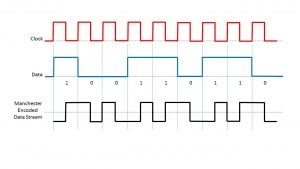
\includegraphics{Diagrams/Manchester_Encoding.jpg}
    \caption{Manchester Encoding}
    \label{fig:encoding}
\end{figure}

\newpage
\noindent\tbox{
    \begin{center}
    \textbf{\Huge Lecture 7}
    \end{center}
}


How to determine the polarity of the signal sent if the voltages are switched. 
The last few bits of the preamble can be dedicated to determining the polarity of the signal. 
Say they are 111, if 111 is received the polarity would be correct and else polarity needs to be flipped. 

However, bit-errors can make this scheme breakdown quickly.

\subsection{Differential Manchester Coding}
Another more error-free option is to encode the messages with Differential Manchester encoding. 
Rules: 
\begin{enumerate}
    \item \textbf{0 bit:} The voltage in the first half of the time period is different from the 
    voltage in the second half of the \textbf{Previous} time period. 
    \item \textbf{1 bit:} The voltage in the first half of the time period is same as the 
    voltage in the second half of the \textbf{Previous} time period.
\end{enumerate}


\section{Phase Modulation in wireless channels}
Wireless signals can be used to represent bits in several ways. 
Frequency, amplitude modulation (ie) encoding the message in values of frequency, amplitude is common. 

However, another popular option is to use phase modulation, (ie) the message is put into the phase of the signal that is sent. 

Unrelated side track:
Since each company has been allocated a band of frequencies available to them. This implies that 
the fourier transform of the signal sent almost completely lies within the appropriate frequency range. 


Assume that \(f_0\) is the centre of this band and the `Bandwidth' is \(2 \Delta\). How do we make sure the 
signal's recieved has a frequency decomposition lying only in the given range? One option is to use a bandpass filter at the receiver end to  
obtain only the signals in some range. 

Take a signal like \(s(t) = A\cos(2\pi ft + \phi)\). The signal recieved would be 
\(\alpha s(t - \delta) + n(t)\). \(\alpha\) is due to attenuation, \(\delta\) is the propogation delay, n(t) is white noise\footnote{White noise is a signal that has energy at all frequencies and cannot be filtered out}(after bandpass filter).

Side track over.
\subsection{Signals as vector spaces}
Signals can actually form a vector space. Each signal is a `vector' offset from 
the axis corresponding to the phase and having length proportional to amplitude.  

The angle between these vectors can be found using their inner product
\[ <a(t),b(t)> = \int_{0}^{T} a(t)b(t) \partial t \]

This can be represented as a 2-d diagram where one axis represents the $\sin$ component of the wave and another the $\cos$ component. 
A phase shifted wave can be represented as a combination of $\sin$, $\cos$ wave. The length of the vector in this domain is proportional to 
amplitude.

This is called the constellation diagram. 

\noindent\tbox{
    \begin{center}
    \textbf{\Huge Lecture 8}
    \end{center}
}


How to get the constellation diagram for a given signal? We can dot the given signal with \(e_x\) and \(e_y\) (ie)
unit normal vectors of this vector space to get each component of the wave. 

Thus given a signal with a phase \(\phi\) its 2d representation can be found to be put on the 
constellation diagram.  

\subsection{BPSK encoding}

Now how do we encode bits using the constellation diagram?

One option is to allocate a region in the 2-d vector space for `1' and another for `0'

Assume that the +x axis points denote signals for bit as `1' and -x axis points denote signals for bit as `0'.
\begin{figure}[H]
    \centering
    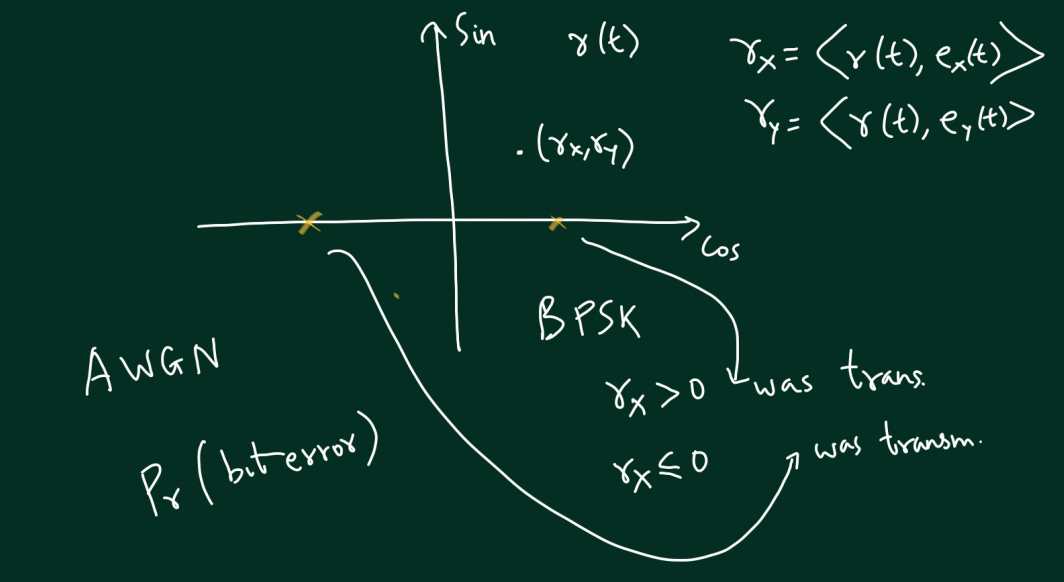
\includegraphics[width = 10cm]{Diagrams/BPSK.png}
\end{figure}

This is called Binary Phase Shift Keying. Note that even with attenuation and 
white noise the amount the received signal shifts in a constellation diagram 
is lesser and thus unlikely to cause a zero to be interpreted as a 1. 


\noindent\tbox{
    \begin{center}
    \textbf{\Huge Lecture 9}
    \end{center}
}
\subsection{QPSK encoding}

The issue with BSPK is that a single signal/wave can only transmit one bit of information.
If we can partition the 2-d plane into say 4 regions and use a similar logic to now assign a 2-bit encoding 
to each region, we can double our throughput. 

This is called Quadrature Phase Shift Keying. One point to be noted is that while 
assigning bits to region it is preferable to assign encoding such that strings which differ in both 
bits are diagonally opposite regions so that even if a misinterpretation does happen its more likely to be a one bit error. 

\begin{figure}
    \centering
    \includegraphics*[width = 10cm]{Diagrams/QPSK.png}
    \caption{Diagram to show bit encoding of each region }
\end{figure}

This idea of more regions being able to encode more bits can be expanded more however 
the more regions it is split into, the more error prone the encoding becomes due the regions being more packed. 
\newpage

\noindent\tbox{
    \begin{center}
    \textbf{\Huge Lecture 10}
    \end{center}
}
\part{Data Link Layer}
\section{Introduction}
The Data link layer deals with preparing a packet to be sent across 
the physical medium and also with error correction in received messages. 

Its exact functionalities are:
\begin{itemize}
    \item \textbf{Framing:} This deals with packaging packets into units called frames by adding headers with the destination MAC address and also some other information, along with redundancies to detect errors. 
    \item \textbf{Error Detection and correction:} When a message is sent there are definite error imposed due to environment. This layer deals with detecting and correcting such errors by adding some redundancy in these messages. 
    \item \textbf{Medium Access:} Deals with managing the shared medium, prevent collisions (where two devices transmit simultaneously), and ensuring fair access for all devices on the network.
\end{itemize}

\subsection{Bit stuffing}

Some networks keep transmitting data in the order of frame, sequence, frame\(\dots\).
A sequence is a filer message sent between two frames. It is the bitstring `01111110'. 

The receiver knows to ignore sequences. However, now the issue is what if an actual message to be sent 
has some substring of the from `01111110'. To deal with this when data is sent every time `11111' (5 1's) appears in a
sequence the next bit is put to be 0. This 0 is removes when the receiver reads a sequence of 5 1's and at the same time 
sequences cannot appear since a sequence of 6 1's is impossible. This insertion of 0`s is called bit stuffing. 


\subsection{Cyclic redundancy check}
Now what if there are bit-flips in the message when it is transmitted?

There is a need to be able to identify and preferable correct some errors. For this purpose 
some extra bits are appended to the end of the message. This is called the Cyclic redundancy check(CRC).

What are some features we would like in CRC?

\begin{itemize}
    \item Want to be easily able to detect a large variety of errors
    \item Creation/verification of this CRC must be efficient
    \item For any n-bit message some k bit CRC should be computable
\end{itemize}


\subsection{Coding Theory}

The process of coming with schemes to create such CRC's is a field called coding theory. 
The basic idea is as follows 
\begin{itemize}
    \item Any n-bit bitstring is mapped to an n+k bitstring
    \item Since there are only \(2^n\) valid bit strings in the n+k bitstring 
    domain an error that results in an invalid string can help us detect an error
    \item Infact given that both sender, receiver know the coding scheme we should be 
    able to map the `defective' n+k bitstring back to the original message. 
\end{itemize}

\subsubsection{Hamming Distance}

Hamming distance between two bitstrings(same length) is the number of bit flips needed to transform one to the other. 
The minimum Hamming distance of a code is the minimum hamming distance between all valid bitstring in the 
n+k bitstring domain explained before. 

\subsubsection{Error Detection:}

If the minimum Hamming distance is N(for a coding scheme), then any 
message with less than \(N-1\) bit errors(but atleast 1) can never be a valid bitstring. If that 
was the case min hamming distance for the code is less than N, which cannot be true. 
\subsubsection{Error Correction:}

If the minimum Hamming distance is 2N + 1 (for a coding scheme), then any 
message with less than \(N-1\) bit errors(but atleast 1) can be mapped to the corresponding corrected bitstring accurately.

This bitstring will be the valid bitstring closest to the one with errors. If that 
was not the case min hamming distance for the code is less than 2N+1, since the bitstring closest to the one with errors 
and the corrected bitstring will have a hamming distance less than 2N+1. 


\noindent\tbox{
    \begin{center}
    \textbf{\Huge Lecture 11}
    \end{center}
}
\subsection{Galois Theory}

A Galois field, named after the mathematician Évariste Galois, is a finite field that contains a set number of elements and supports operations of addition, subtraction, multiplication, and division (excluding division by zero). 

We define a galois field where addition is replaced by xor. 

The claim is that for any given data bit string, the remainder obtained when the data(appended with k zeros) is divided\footnote{Not exactly but similar operation} by 
a special k+1 bit generator gives us a CRC. 

\textbf{Example:}

Data is `110110', generator is `1101'. 
Note that here there is no carry in the addition, just bit by bit addition. 

\begin{figure}[H]
    \centering
    \includegraphics*[width = 10cm]{Diagrams/galois.jpg}
    \caption{Example for CRC generation}   
\end{figure}

So the algorithm is similar to long division and just uses additions one after another instead of 
subtraction. 

This algorithm can in fact be simulated by a simple logic circuit. 


How can this CRC be used for error correction at the receiver side?
\begin{itemize}
    \item If the received message on divison with the generator does not give 000 as a remainder then there is an error
    \item Take the data part of the message and append 000 to it and perform division with the generator. If the remainder obtained from this does not match with the CRC there was an error in the transmission
\end{itemize}

\noindent\tbox{
    \begin{center}
    \textbf{\Huge Lecture 12}
    \end{center}
}
\section{Polynomial Arithmetic}

As done before in Galois fields, division is still defined using 
Addition (xor), multiplication (normal).

But encoding is now being done as the coeffiicent of Polynomials. 
For example, something like `110110' is encoded as \(x^5 + x^4 + x^2 + x\). 
In this context what does it mean for \(A(x)\) to be divisble by \(D(x)\), basically

\[A(x) = B(x)D(x)\]

Let's try to understand how to use this now, 

Say \(P(x)\) is the message to be sent (clear from before Polynomial is equivalent to bitstrings), lets say some bits get 
flipped in the Polynomial. The bits that get flipped corresponds to a polynomial \(E(x)\). 


So the total received message can be denoted as \(P(x) + E(x)\). 
Now if the generator is known across both devices which have the message and it also divides \(P(x)\), then 
error detection can be done by checking if \(P(x) + E(x)\) is divisible by \(C(x)\). 

For this method to work, \(E(x)\) cannot be divisible by \(C(x)\). But is this the case?

\begin{itemize}
    \item \textbf{Single Error Bit:} E(x) = \(x^i\) for some i,
    Suppose \(C(x) = x^k + 1\)
    then \(C(x)\) cannot divide \(E(x)\), 

    To see why think of a divisor for this operation, say \(D(x)\)
    \begin{align}
        C(x) D(x) &= x^i \\
        (x^n + \dots + 1)(x^m + \dots + x^q) &= x^i
    \end{align}

    The above is not possible.

    \item \textbf{Two Bit Errors:} 
    \(E(x) = x^j + x^i\), (j $>$ i)
    \(E(x) = x^i(x^{j-i} + 1)\)
    
    Suppose \(C(x)\) is of the form \(x^k + \dots + 1\)

    Now again the problem reduces to if \(C(x)\) can divide \(P(x) + E(x)\), which 
    basically is asking if it can divide \(E(x)\). 

    \textbf{Order of a Polynomial:} The smallest `r' such that \(C(x)\) divides \(x^r + 1\) is called its order. 
    
    Methods are known to find \(C(x)\) such that their orders are very high. 
    \textbf{Example:} k = 16, \(C(x) = x^{16} + \dots + 1\), then we can find \(c(x)\) s.t it will
    not divide any \(x^p + 1\), if \(p < 2^{16} - 1\). 

    \item \textbf{Odd number of Errors:}
    \begin{enumerate}
        \item If \(C(x) = (1+x)(...)(...)\), this can catch all odd number of errors.
        \item If \(C(x)\) has even number of terms, it can also capture all odd number of errors. 
    \end{enumerate}
    Why is this true?
    \begin{enumerate}
        \item Assume that a Polynomial \(E(x)\) has an odd number of terms, \(E(1)\) is `1', since addition is xor.
        Similary \(C(1)\) is 0. Since the term \(1 + 1\) becomes 0. 

        Thus \(E(x)\)*\(D(x)\) = \(C(x)\) can never be true since the equation fails for \(x = 1\).
        
        \item Similar argument applies to argue that \(C(1)\) is 0 when it has even number of terms.  
    \end{enumerate}

    \item \textbf{Burst of Errors:}
    Many times, due to interference we have a consecutive sequence of bits which get flipped. 

    Thus \[E(x) = x^{i + l -1} + x^{i + l -2} + \dots + x^i\], which can also be 
    written as \((x^i)(x^{l-1} + x^{l-2} + \dots+ 1)\)

    If our carry is of form \(C(x) = x^k + x^{k-1} + x^{k-2} + \dots + 1\). 
    It can detect all burst errors of length less than l, since it cannot divide the error term. 
    If you are not convinced think of a dividend \(D(x)\) then \(E(x) = C(x)D(x)\), which is not possible. 
\end{itemize}
\subsection{Some Polynomial CRC's}

CRC-32: \(x^{32} + x^{26} + x^{23} + x^{22} + x^{16} + x^{12} + x^{11} + x^{10} + x^{8} + x^{7} + x^{5} + x^{4} + x^{2} + x + 1 \)


\noindent\tbox{
    \begin{center}
    \textbf{\Huge Lecture 13}
    \end{center}
}
\section{Media Access Control}

Media Access Control protocol takes care of managing shared resources over a network. It helps 
a device access the medium of communication (a wire, wireless tower) in-order to start transmitting data. 
The protocol manages which device has control over the shared media so that multiple people don't use the network at once and thus 
start to interfere with one another. 

Also, there is a need for each need for each message to be addressed to the destination so that 
the message can reach the receiver accurately, which is also taken care of by the MAC.

One way to do this is to give a particular frequency bandwidth to each device as an identifier. 
However, this method cannot easily accommodate the addition of new devices. Further it hampers the Bandwidth of the network as more 
devices split up the available bandwidth.  
To enable this functionality, the MAC protocol requires that each `Network Interface Card (NIC)' has a
unique MAC address. This is taken care by the manufacturer and hard coded into the card. 

MAC address come out of the size of 48 bits, so for the reasonable future we have enough address to get a MAC
address for all cards. 


\subsection{Interference}

What about interference? If it can be ensured that only one device uses the network at one time, then 
interference is taken care of. 

Possible methods:
\begin{itemize}
    \item \textbf{Frequency-Based:} Will different frequencies help? How to allocate different frequencies to devices? This method however still has the Bandwidth issue mentioned earlier. 
    \item \textbf{Time-Based:} A leader device can be assigned such that it sends a special message to send to a device
    to indicate that it is their turn to send a message. The issue is that 
    if A doesn't use a time slot then that time is wasted. 
    \item \textbf{Token-Based:} There is a `token' message the owner of which is allowed to transfer messages. A 
    token release message is sent if a particular device passes the token to the next device. The token release message has 
    a identifier for the device which is going to receive the token. 

    A common form of implementing the token system is to connect devices in a ring topology and have the 
    token sent from one device to the next in a step by step fashion. In this system fairness is maintained since 
    each system gets an opportunity to transmit its message within one cycle. 

\end{itemize}

The second one is a better option in some ways since it completely negates interference. A smart leader can also 
assign more time slots to a device if it sends a message with many packets.



\noindent\tbox{
    \begin{center}
    \textbf{\Huge Lecture 14}
    \end{center}
}
\subsubsection{Frequency and time}

There is a possibility to combine both frequency and time based methods to prevent 
interference. Note that this is also a leader based system and we call the leader the `base station'. 

Say a particular frequency band is assigned to a company\footnote{This is called a frame}. This band can 
be split up into further smaller bands called sub-channels. Now these sub-channels can be further divided into time 
chunks to entirely split up the frequency * time domain into a grid. 


How to decide who uses which block in the grid? The base station sends a scheduling message before transmission
to denote which frequency and time slot is used for which message. 

Any user first synchronises with the base station for purposes like syncing up this clock. So they also 
receive this scheduling message once they connect with the base station. 

What is the point of all this hassle over simple time sharing? 
Well clearly more information can be pumped through the system compared to when there is only 
one user per time slot. 


\textbf{Down-link:} When user receives data from the base station

\textbf{Up-link:} User sends data to the base station


\subsubsection{Issues with Central Coordinator}
\begin{itemize}
\item Single point of failure
\item May not be possible in certain situations (when the bandwidth is unlicensed)
\end{itemize}
\subsection{No central coordinator}

What are the wants from such a system?
\begin{itemize}
    \item \textbf{Plug and play:} need to be able to connect and disconnect any device from the network
    \item No central coordinator exists
\end{itemize}


How to prevent interference without a coordinator?

The idea is that if only one node transmits most of the time, then we rarely have collisions. 
Why is a collision so bad? When multiple nodes transfer messages at the same time, they all interfere and become 
meaningless and cannot be split up. 

Main idea \(\rightarrow\) If there is a collision detected then stop transmitting. How to detect collisions?
Since the combined signal will have a much higher energy, a collision can be detected by this increase in energy. 


\begin{figure}[H]
    \centering
    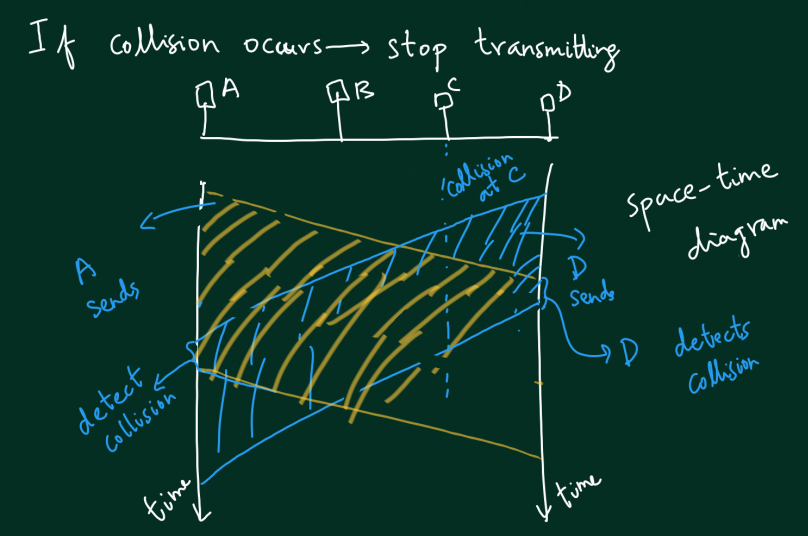
\includegraphics[width=10cm]{Diagrams/collision.png}
\end{figure}


\end{document}